\chapter{Neurónové siete}

\iffalse
Formálne  je neurónová    sieť    určená    ako    orientovaný    graf    G=(V,E).    
Výrazy V={v1,v2,...,vN}  a  E={e1,e2,...eM}  označujú  neprázdnu  vrcholovú  množinu  resp.  hranovú množinu grafu G obsahujúceho N vrcholov (neurónov) a M hrán (spojov). Každý spoj $e \in E$ sa interpretuje ako usporiadaná dvojica dvoch neurónov z množiny V, e=(v,v’).  
Hovoríme, že  spoj  e  začína  v  neuróne  v  a  končí  v  neuróne  v’.  Množina  neurónov  V  je  rozložená  na disjunktné podmnožiny.

kde VI obsahuje NI vstupných neurónov, ktoré sú susedné len s vychádzajúcimi hranami, VH obsahuje NH skrytých (angl. hidden) neurónov, ktoré sú susedné súčasne  s  vychádzajúcimi ako aj s vchádzajúcimi hranami, a konečne VO obsahuje NO výstupných neurónov, ktoré súsusedné  len  s  vchádzajúcimi  hranami.  
V  našich  nasledujúcich  úvahách  budeme  vždy predpokladať,  že  množiny  VI  a  VO  sú  neprázdne,  t.j.  neurónová  sieť  obsahuje  vždy  aspoň jeden vstupný a jeden výstupný neurón.
Pre acyklické neurónové siete (ktoré neobsahujú orientované cykly neuróny môžu byť usporiadané do vrstiev VL  L  $LL=\cup \cup \cup \cup 12 3...t$, kde L1=VI je vstupná vrstva (obsahuje len vstupné neuróny), L2, L3,..., Lt–1 sú skryté vrstvya  Lt  je  výstupná  vrstva.  
Vrstva  Li  (pre  $1\leq i\leq t$)  je  určená  nasledujúcim  jednoduchým spôsobom $LVivdvi=\in   =+;aflq1$, kde vzdialenosť d(v) sa rovná dĺžke maximálnej cesty, ktorá spája daný neurón so vstupným neurónom, potom musí platiť d(v)=0, pre $v\in VI$. 
Neurónová sieť určená acyklickým grafom je  obvykle  volená  tak,  že  neuróny  z  dvoch  susedných  vrstiev  sú  poprepájané  všetkými možnými  spojmi.  
Žiaľ,  takýto  rozklad  množiny  neurónov  na  vrstvy  je Obrázok 5.2. 
Neurónová sieť je definovaná ako orientovaný súvislý graf. 
Diagram A obsahuje orientovaný graf  s  jedným  cyklom  a  teda  nemôže  byť  použitý  pre  definíciu  neurónovej  siete  s  dopredným  šírením.
Diagram  B  ilustruje  možnosť  rozkladu  vrcholov  (neurónov)  acyklického  orientovaného  grafu  na  vrstvy L1,..,L4.
kde L1=VI je vstupná vrstva (obsahuje len vstupné neuróny), L2, L3,..., Lt–1 sú skryté vrstvya  Lt  je  výstupná  vrstva.  Vrstva  Li  (pre  $1\leq i\leq t$)  je  určená  nasledujúcim  jednoduchýmspôsobom$LVivdvi=\in   =+$;aflq1                                  (5.9)kde vzdialenosťd(v) sa rovná dĺžke maximálnej cesty, ktorá spája daný neurón so vstupnýmneurónom, potom musí platiťd(v)=0, pre $v\in VI$. Neurónová sieť určená acyklickým grafomje  obvykle  volená  tak,  že  neuróny  z  dvoch  susedných  vrstiev  sú  poprepájané  všetkýmimožnými  spojmi  (pozri  obr.  5.3). \citep{rnn:spol}

\fi

Neurónová sieť je založená na orientovanom grafe (ako je možné vidieť na obrázku \ref{fig:nn}), je teda zložená z uzlov, ktoré sú spojené orientovanými hranami \citep{rnn:spol}.
Spojenie uzlu $i$ do uzlu $j$ slúži na propagáciu aktivácie $a_i$ z $i$ do $j$.
Každé takéto spojenie má priradenú váhu $w_{i,j}$, ktorá rozhoduje o sile a znamienku spojenia.
Každý uzol má naviac falošný vstup $a_0=1$ s priradenou váhou $w_{0,j}$.
Všetky uzly si potom vypočítajú váženú hodnotu vstupov, pre uzol $j$ je táto hodnota:
$$in_j=\sum^n_{i=0}w_{i,j}a_i$$
Potom sa na výsledok aplikuje aktivačná funkcia g, tým získame výstup z uzlu:
$$a_j=g(in_j)=g\left(\sum^n_{i=0}w_{i,j}a_i\right)$$

\begin{figure} \label{fig:nn}
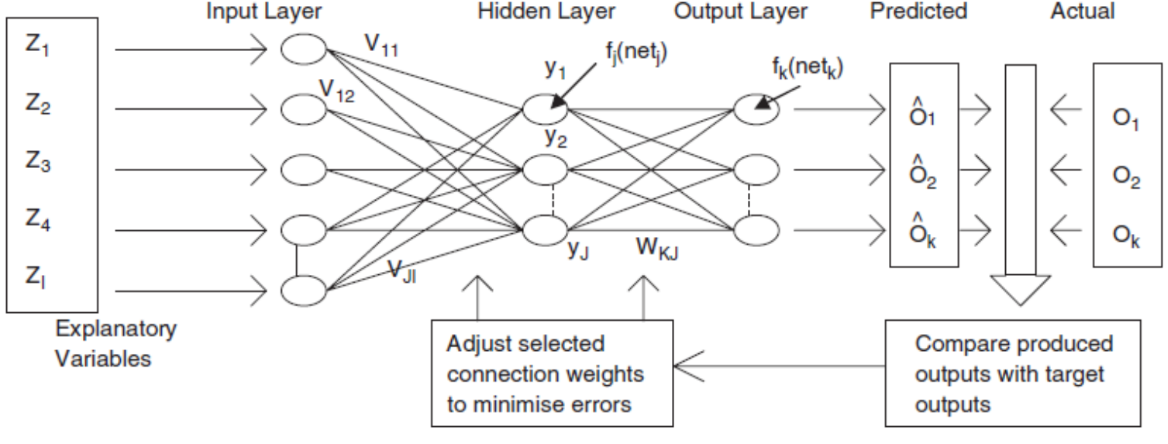
\includegraphics[width=\textwidth]{../img/nn.png}
\caption{Na obrázku je ukážka jednej z neurónových sietí. Konkrétne to je sieť, ktorú použili v roku 2014 iránski výskumníci pri predikcii výsledkov najvyššej iránskej ligy \citep{related:iran}.}
\end{figure}

Aktivačná funkcia $g$ je typicky buď pevná hranica alebo logistická funkcia.
V prvom prípade sa uzly volajú perceptrony, v druhom prípade sa niekedy používa pojem sigmoid perceptron.
Obe tieto typy nelineárnych aktivačných funkcií zaručujú dôležitú vlastnosť neurónovej siete, a to, že celá sieť uzlov môže reprezentovať aj nelineárnu funkciu.

\begin{figure}
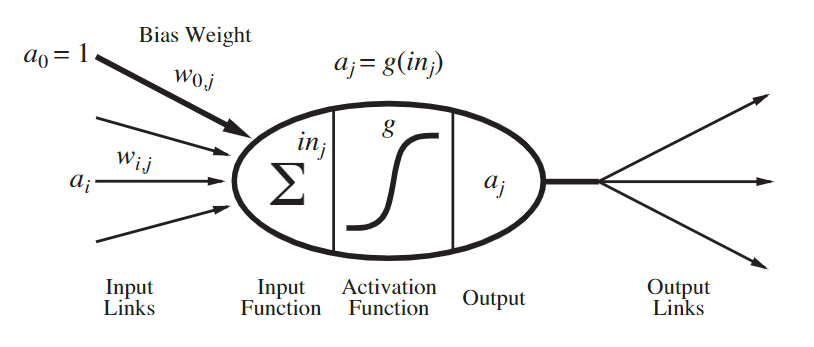
\includegraphics[width=\textwidth]{../img/nn_aima_neuron.png}
\caption{Takto vyzerá jeden uzol siete (neurón) \citep{aima}.}
\end{figure}

Takto teda vyzerá matematický model jedného uzlu (v tomto prípade zvaného neurón) v sieti.
Spájanie týchto neurónov vytvorí sieť.
Existujú dva rozdielne prístupy, akými sa dajú tieto neuróny spojiť do siete. 
Obe nás zaujímajú pre túto prácu, pretože obe použijeme v praxi a budeme ich porovnávať medzi sebou.

Neurónové siete sú obvykle zoradené do vstiev tak, že každý neurón dostane vstup len z neurónov z predošlej vrstvy.
Podľa počtu vrstiev sa siete delia na jednovrstvové a viacvrstvové, kde jednovrstvové siete spájajú vstpné neuróny priamo s výstupnými.
Viacvrstvové siete majú medzi vstupom do siete a výstupom z nej ešte jednu alebo viac vrstiev tzv. skrytých (hidden) neurónov (Obrázok \ref{img:single}) \citep{aima}.

\begin{figure} \label{img:single}
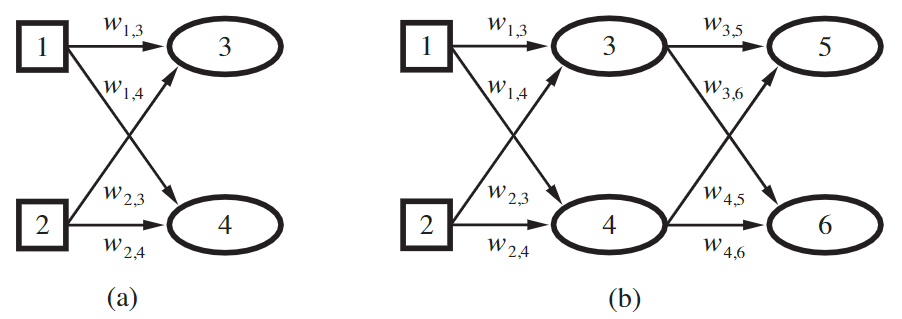
\includegraphics[width=\textwidth]{../img/nn_aima_single_multi.png}
\caption{Ukážka rozdielu medzi jednovrstvou sieťou (a) a viacvrstvovou (b). Obe majú 2 vstupné a 2 výstupné neuróny, viacvrstvová má ešte medzi nimi ďalšie vrstvy skrytých neurónov (v tomto prípade jednu vrstvu s 2 skrytými neurónmi) \citep{aima}.}
\end{figure}

\section{Dopredné neurónové siete}
Dopredná neurónová sieť (feed-forward neural network) má spojenia len v jednom smere, takže tvorí orientovaný acyklický graf.
Ak si graf topologicky usporiadame, tak každý uzol dostane vstup z niektorých z predchádzajúcich uzlov a predá výstup niektorým z nasledujúcich vrcholov.
Dopredná neurónová sieť teda predstavuje funkciu jej momentálneho vstupu, teda neuchováva žiaden stav, ak nepočítame váhy samotné \citep{aima}.

\section{Rekurentné neurónové siete}
Na druhej strane je rekurentná neurónová sieť (recurrent neural network).
Tento typ siete posúva svoj výstup naspäť do svojho vlastného vstupu. 
Z toho vyplýva, že aktivačné úrovne siete tvoria dynamický systém, ktorý môže dosiahnuť stabilný stav alebo oscilovať či sa dokonca správať chaoticky.

Výstup siete závisí na vstupe. 
Pri tomto type siete môže výstup závisieť aj na predchádzajúcich výstupoch, tranzitívne teda aj na predchádzajúcich vstupoch.
Z toho vyplýva, že si rekurentná neurónová sieť môže vypracovať krátkodobú pamäť \citep{aima}.